%% USPSC-TCC-modelo.tex
% ---------------------------------------------------------------
% USPSC: Modelo de Trabalho Academico (tese de doutorado, dissertacao de
% mestrado e trabalhos monograficos em geral) em conformidade com 
% ABNT NBR 14724:2011: Informacao e documentacao - Trabalhos academicos -
% Apresentacao
%----------------------------------------------------------------
%% Esta é uma customização do abntex2-modelo-trabalho-academico.tex de v-1.9.5 laurocesar 
%% para as Unidades do Campus USP de São Carlos:
%% EESC - Escola de Engenharia de São Carlos
%% IAU - Instituto de Arquitetura e Urbanismo
%% ICMC - Instituto de Ciências Matemáticas e de Computação
%% IFSC - Instituto de Física de São Carlos
%% IQSC - Instituto de Química de São Carlos
%%
%% Este trabalho utiliza a classe USPSC.cls que é mantida pela seguinte equipe:
%% 
%% Coordenação e Programação:
%%   - Marilza Aparecida Rodrigues Tognetti - marilza@sc.usp.br (PUSP-SC)
%%   - Ana Paula Aparecida Calabrez - aninha@sc.usp.br (PUSP-SC)
%% Normalização:
%%   - Brianda de Oliveira Ordonho Sigolo - brianda@usp.br (IAU)
%%   - Eduardo Graziosi Silva - edu.gs@sc.usp.br (EESC)
%%   - Eliana de Cássia Aquareli Cordeiro - eliana@iqsc.usp.br (IQSC)
%%   - Flávia Helena Cassin - cassinp@sc.usp.br (EESC)
%%   - Maria Cristina Cavarette Dziabas - mcdziaba@ifsc.usp.br (IFSC)
%%   - Regina Célia Vidal Medeiros - rcvmat@icmc.usp.br (ICMC)
%%
%% O USPSC-modelo.tex e USPSC-TCC-modelo.tex utilizam diversos arquivos relacionado em 
%% 2.1 Pacote USPSC: Classe USPSC e modelos de trabalhos acadêmicos	do Tutorial do Pascote 
%%  USPSC para modelos de trabalhos de acadêmicos em LaTeX - versão 3.1


%----------------------------------------------------------------
%% Sobre a classe abntex2.cls:
%% abntex2.cls, v-1.9.5 laurocesar
%% Copyright 2012-2015 by abnTeX2 group at https://www.abntex.net.br/ 
%%
%----------------------------------------------------------------

\documentclass[
% -- opções da classe memoir --
12pt,		% tamanho da fonte
openright,	% capítulos começam em pág ímpar (insere página vazia caso preciso)
twoside,  % para impressão em anverso (frente) e verso. Oposto a oneside - Nota: utilizar \imprimirfolhaderosto*
%oneside, % para impressão em páginas separadas (somente anverso) -  Nota: utilizar \imprimirfolhaderosto
% inclua uma % antes do comando twoside e exclua a % antes do oneside 
a4paper,			% tamanho do papel. 
% -- opções da classe abntex2 --
chapter=TITLE,		% títulos de capítulos convertidos em letras maiúsculas
% -- opções do pacote babel --
english,			% idioma adicional para hifenização
french,				% idioma adicional para hifenização
spanish,			% idioma adicional para hifenização
brazil				% o último idioma é o principal do documento
% {USPSC-classe/USPSC} configura o cabeçalho contendo apenas o número da página
]{USPSC-classe/USPSC}
%]{USPSC-classe/USPSC1}
% Inclua % antes de ]{USPSC-classe/USPSC} e retire a % antes de %]{USPSC-classe/USPSC1} para utilizar o 
% cabeçalho diferenciado para as páginas pares e ímpares:
%- páginas ímpares: com seções ou subseções e o número da página
%- páginas pares: com o número da página e o título do capítulo 
% ---
% ---
% Pacotes básicos - Fundamentais 
% ---
\usepackage[T1]{fontenc}		% Seleção de códigos de fonte.
\usepackage[utf8]{inputenc}		% Codificação do documento (conversão automática dos acentos)
\usepackage{lmodern}			% Usa a fonte Latin Modern
% Para utilizar a fonte Times New Roman, inclua uma % no início do comando acima  "\usepackage{lmodern}"
% Abaixo, tire a % antes do comando  \usepackage{times}
%\usepackage{times}		    	% Usa a fonte Times New Roman	
% Para usar a fonte , lembre-se de tirar a % do comando %\renewcommand{\ABNTEXchapterfont}{\rmfamily}, localizado mais abaixo, logo após "Outras opções para nota de rodapé no Sistema Numérico" 					
\usepackage{lastpage}			% Usado pela Ficha catalográfica
\usepackage{indentfirst}		% Indenta o primeiro parágrafo de cada seção.
\usepackage{color}				% Controle das cores
\usepackage{graphicx}			% Inclusão de gráficos
\usepackage{float} 				% Fixa tabelas e figuras no local exato
\usepackage{tikz}				% Para escrever reações químicas e outros
\usetikzlibrary{positioning}
\usepackage{microtype} 			% para melhorias de justificação
\usepackage{pdfpages}
\usepackage{makeidx}            % para gerar índice remissivo
\usepackage{hyphenat}          % Pacote para retirar a hifenizacao do texto
\usepackage[absolute]{textpos} % Pacote permite o posicionamento do texto
\usepackage{eso-pic}           % Pacote para incluir imagem de fundo
\usepackage{makebox}  
\usepackage{amsmath}
% Pacote para criar caixa de texto
% ---

% ---
% Pacotes de citações
% Citações padrão ABNT
% ---
% Sistemas de chamada: numérico.

% Sistema Numérico
% Para citações numéricas, sistema adotado pelo IFSC, incluir % no início dos comandos acima e retirar a % dos comandos abaixo 
\usepackage[superscript]{cite}              % agrupa citações numéricas consecutivas
\usepackage[num, abnt-emphasize=bf, abnt-thesis-year=both, abnt-repeated-author-omit=no, abnt-last-names=abnt, abnt-etal-cite, abnt-etal-list=3, abnt-etal-text=it, abnt-and-type=e, abnt-doi=doi, abnt-url-package=none, abnt-verbatim-entry=no]{abntex2cite} 
\bibliographystyle{USPSC-classe/abntex2-num-USPSC}

% Complementarmente, verifique as instruções abaixo sobre os Pacotes de Nota de rodapé
% ---
% Pacotes de Nota de rodapé
% Configurações de nota de rodapé

% O presente modelo adota o formato numérico para as notas de rodapés quando utiliza o sistema de chamada autor-data para citações e referências. Para utilizar o sistema de chamada numérico para citações e referências, habilitar um dos comandos abaixo.
% Há diversa opções para nota de rodapé no Sistema Numérico.  Para o IFSC, habilitade o comando abaixo.

\renewcommand{\thefootnote}{\fnsymbol{footnote}}  %Comando para inserção de símbolos em nota de rodapé

\renewcommand{\footnotesize}{\small} %Comando para diminuir a fonte das notas de rodapé

% ---
% Pacote para agrupar a citação numérica consecutiva
% Quando for adotado o Sistema Numérico, a exemplo do IFSC, habilite 
% o pacote cite abaixo retirando a porcentagem antes do comando abaixo
%\usepackage[superscript]{cite}	

% ---
% Pacotes adicionais, usados apenas no âmbito do Modelo Canônico do abnteX2
% ---
\usepackage{lipsum}				% para geração de dummy text
% ---

% pacotes de tabelas
\usepackage{multicol}	% Suporte a mesclagens em colunas
\usepackage{multirow}	% Suporte a mesclagens em linhas
\usepackage{longtable}	% Tabelas com várias páginas
\usepackage{threeparttablex}    % notas no longtable
\usepackage{array}

\usepackage{physics}
\usepackage{bbold}
\usepackage{subcaption}

% ----
% Compatibilização com a ABNT NBR 6023:2018
% Para tirar <> da URL
%\DeclareFieldFormat{url}{\bibstring{urlfrom}\addcolon\addspace\url{#1}}
\usepackage{USPSC-classe/ABNT6023-2018}
% As demais compatibilizações estão nos arquivos abntex2-alf-USPSC.bst,abntex2-alfeng-USPSC.bst, abntex2-num-USPSC.bst e abntex2-numeng-USPSC.bst, dependendo do idioma do textos e se o sistemas de chamada for autor-data ou numérico, conforme explicitado acima.
% ----

% ---
% DADOS INICIAIS - Define sigla com título, área de concentração e opção do Programa 
% Consulte a tabela referente aos Programas, áreas e opções de sua unidade contante do
% arquivo USPSC-Siglas estabelecidas para os Programas de Pós-Graduação por Unidade.xlsx 
% ou nos APÊNDICES A-F
\siglaunidade{IFSC-TCC}
\programa{BFCp}
% Os demais dados deverão ser fornecidos no arquivo USPSC-pre-textual-UUUU ou USPSC-TCC-pre-textual-UUUU, onde UUUU é a sigla da Unidade. 
% Exemplo:USPSC-pre-textual-IFSC.tex
% ---'
% Configurações de aparência do PDF final
% alterando o aspecto da cor azul
\definecolor{blue}{RGB}{41,5,195}




% informações do PDF
\makeatletter
\hypersetup{
	%pagebackref=true,
	pdftitle={\@title}, 
	pdfauthor={\@author},
	pdfsubject={\imprimirpreambulo},
	pdfcreator={LaTeX with abnTeX2},
	pdfkeywords={abnt}{latex}{abntex}{USPSC}{trabalho acadêmico}, 
	colorlinks=true,       		% false: boxed links; true: colored links
	linkcolor=black,          	% color of internal links
	citecolor=black,        		% color of links to bibliography
	filecolor=black,      		% color of file links
	urlcolor=black,
	%Para habilitar as cores dos links, retire a % antes dos comandos abaixo e inclua a % antes das 4 linhas de comando acima 
	%linkcolor=blue,            	% color of internal links
	%citecolor=blue,        		% color of links to bibliography
	%filecolor=magenta,      		% color of file links
	%urlcolor=blue,
	bookmarksdepth=4	
}
\makeatother
% --- 
% --- 
% Espaçamentos entre linhas e parágrafos 
% --- 

% O tamanho do parágrafo é dado por:
\setlength{\parindent}{1.3cm}

% Controle do espaçamento entre um parágrafo e outro:
\setlength{\parskip}{0.2cm}  % tente também \onelineskip

% ---
% compila o sumário e índice
\makeindex
% ---

% ----
% Início do documento
% ----
\begin{document}

% Seleciona o idioma do documento (conforme pacotes do babel)
\selectlanguage{brazil}
% Se o idioma do texto for inglês, inclua uma % antes do 
%      comando \selectlanguage{brazil} e 
%      retire a % antes do comando abaixo
%\selectlanguage{english}

% Retira espaço extra obsoleto entre as frases.
\frenchspacing 

% --- Formatação dos Títulos
\renewcommand{\ABNTEXchapterfontsize}{\fontsize{12}{12}\bfseries}
\renewcommand{\ABNTEXsectionfontsize}{\fontsize{12}{12}\bfseries}
\renewcommand{\ABNTEXsubsectionfontsize}{\fontsize{12}{12}\normalfont}
\renewcommand{\ABNTEXsubsubsectionfontsize}{\fontsize{12}{12}\normalfont}
\renewcommand{\ABNTEXsubsubsubsectionfontsize}{\fontsize{12}{12}\normalfont}


% ----------------------------------------------------------
% ELEMENTOS PRÉ-TEXTUAIS
% ----------------------------------------------------------
% ---
% Capa
% ---
\imprimircapa
% ---
% Folha de rosto
% (o * indica impressão em anverso (frente) e verso )
% ---
\imprimirfolhaderosto*
%\imprimirfolhaderosto
% ---
% ---
% Inserir a ficha catalográfica em pdf
% ---
% A biblioteca da sua Unidade lhe fornecerá um PDF com a ficha
% catalográfica definitiva. 
% Quando estiver com o documento, salve-o como PDF no diretório
% do seu projeto como fichacatalografica.pdf e inclua o arquivo
% utilizando o comando abaixo:

%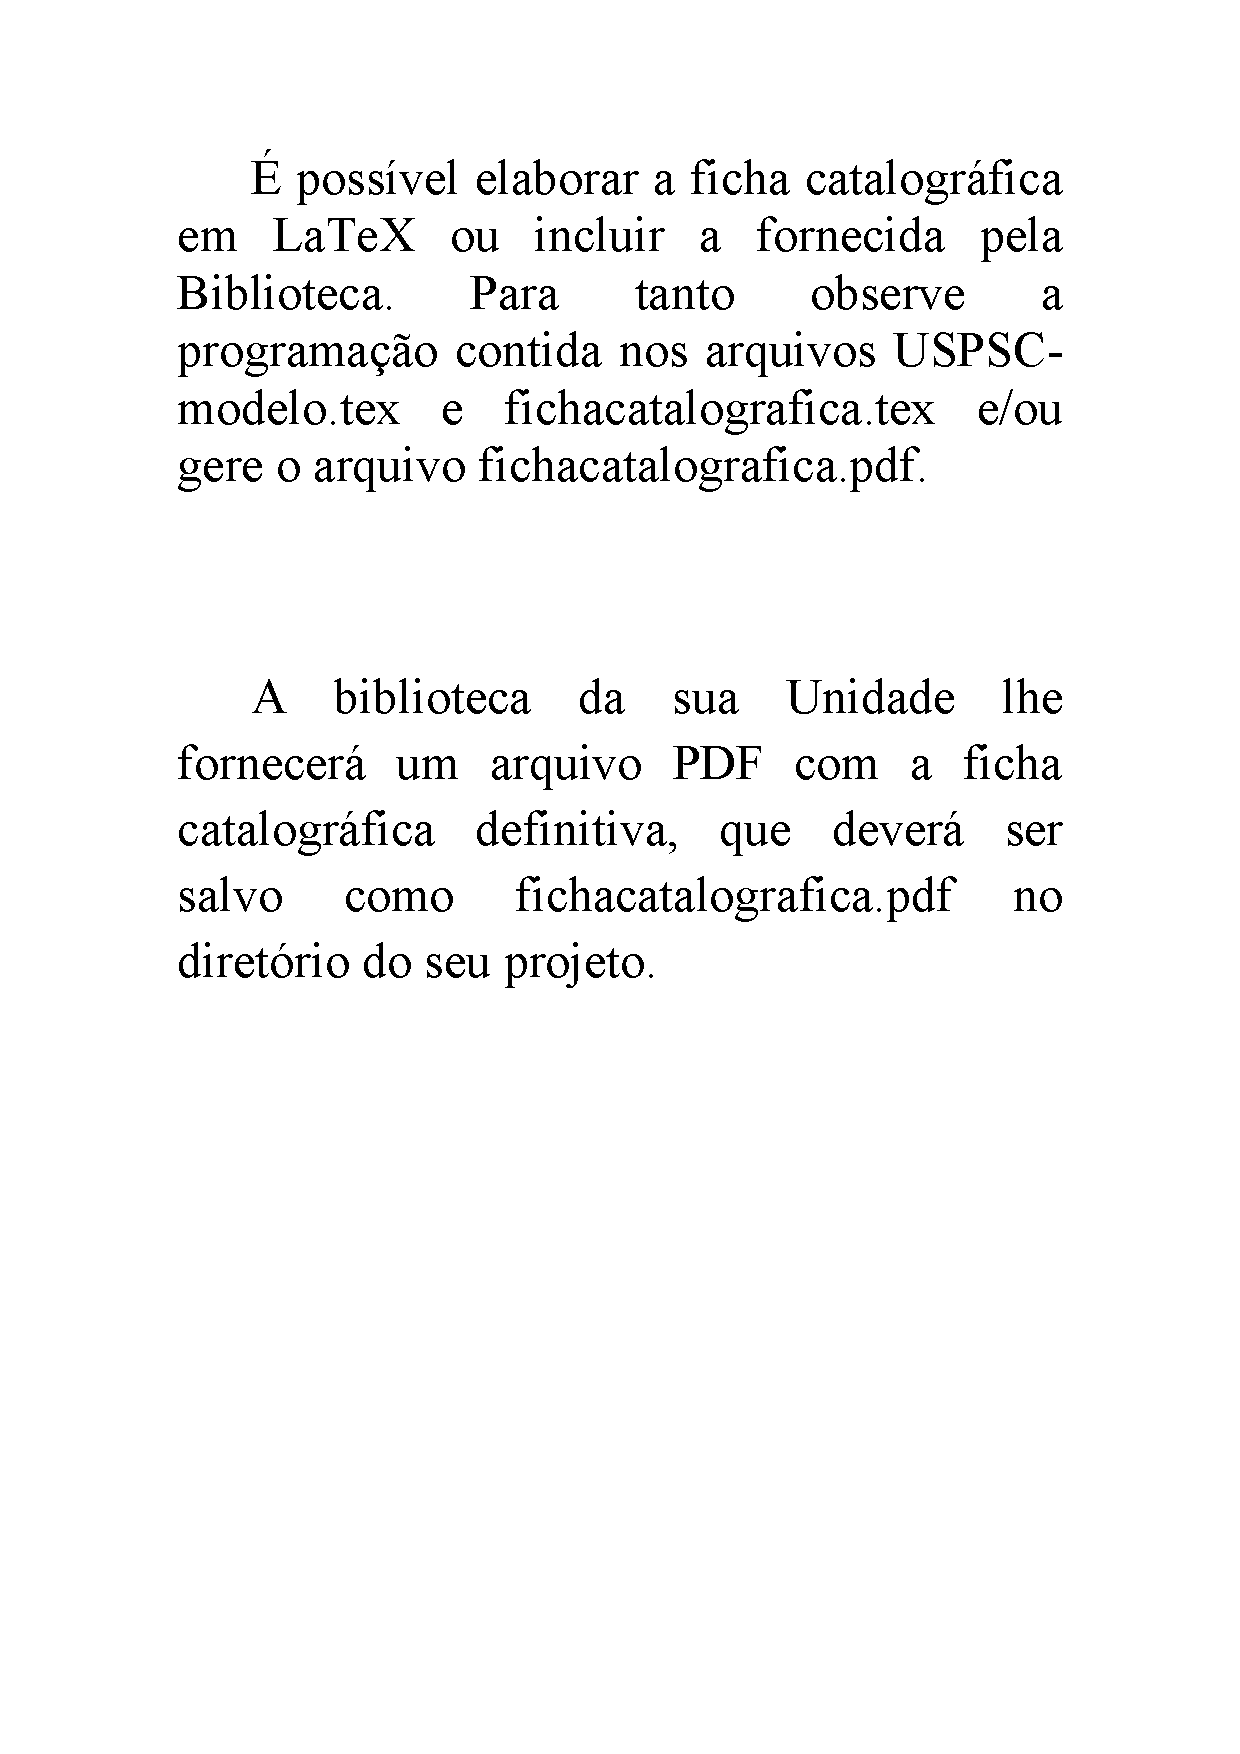
\includepdf{USPSC-TA-PreTextual/USPSC-fichacatalografica.pdf}

% Se você optar por elaborar a ficha catalográfica, deverá 
% incluir uma % antes da linha % antes
% do comando %% USPSC-fichacatalografica.tex
% ---
% Inserir a ficha bibliografica
% ---
% Isto é um exemplo de Ficha Catalográfica, ou ``Dados internacionais de
% catalogação-na-publicação''. Você pode utilizar este modelo como referência. 
% Porém, provavelmente a biblioteca da sua universidade lhe fornecerá um PDF
% com a ficha catalográfica definitiva após a defesa do trabalho. Quando estiver
% com o documento, salve-o como PDF no diretório do seu projeto e substitua todo
% o conteúdo de implementação deste arquivo pelo comando abaixo:
%
\begin{fichacatalografica}
	\hspace{-1.4cm}
	\imprimirnotaautorizacao \\ \\
	%\sffamily
	\vspace*{\fill}					% Posição vertical
\begin{center}					% Minipage Centralizado
  \imprimirnotabib \\
  \begin{table}[htb]
	\scriptsize
	\centering	
	\begin{tabular}{|p{0.9cm} p{8.7cm}|}
		\hline
	      & \\
		  &	  \imprimirautorficha     \\
		
		 \imprimircutter & 
							\hspace{0.4cm}\imprimirtitulo~  / ~\imprimirautor~ ;  ~\imprimirorientadorcorpoficha. -- 	\imprimirlocal, \imprimirdata.   \\
		
		  &  % Para incluir nota referente à versão corrigida no corpo da ficha,
			  % incluir % no início da linha acima e tirar a % do início da linha abaixo
			  %	\hspace{0.4cm} \imprimirtitulo~  / ~\imprimirautor~ ; ~\imprimirorientadorcorpoficha~- ~\imprimirnotafolharosto. -- \imprimirlocal, \imprimirdata.  \\
		
			\hspace{0.4cm}\pageref{LastPage} p.\\ 
		  & \\
		  & 
		    \hspace{0.4cm}\imprimirnotaficha ~--~ 
						  \imprimirunidademin, 
						  \imprimiruniversidademin, 
		                  \imprimirdata. \\ 
		  & \\                 
		   % Para incluir nota referente à versão corrigida em notas,
		    % incluir uma % no início da linha acima e	
		    % tirar a % do início da linha abaixo
		    % & \hspace{0.4cm}\imprimirnotafolharosto \\ 
		  & \\ 
		  & \hspace{0.4cm}1. Introdução. 2. Matrizes Aleatórias. 3. Simulações e Algoritmos. 4. Implementação e Resultados 5. Conclusão. I. \imprimirorientadorficha. II. Matrizes Aleatórias e Simulação de Gases de Coulomb. \\
	
		     %Se houver co-orientador, inclua % antes da linha (antes de II. Título.) 
		     %          e tire a % antes do comando abaixo 
		     %III. Título. \\   
		  \hline
	\end{tabular}
  \end{table}
\end{center}
\end{fichacatalografica}
% ---

 
% e retirar o % do comando abaixo
%% USPSC-fichacatalografica.tex
% ---
% Inserir a ficha bibliografica
% ---
% Isto é um exemplo de Ficha Catalográfica, ou ``Dados internacionais de
% catalogação-na-publicação''. Você pode utilizar este modelo como referência. 
% Porém, provavelmente a biblioteca da sua universidade lhe fornecerá um PDF
% com a ficha catalográfica definitiva após a defesa do trabalho. Quando estiver
% com o documento, salve-o como PDF no diretório do seu projeto e substitua todo
% o conteúdo de implementação deste arquivo pelo comando abaixo:
%
\begin{fichacatalografica}
	\hspace{-1.4cm}
	\imprimirnotaautorizacao \\ \\
	%\sffamily
	\vspace*{\fill}					% Posição vertical
\begin{center}					% Minipage Centralizado
  \imprimirnotabib \\
  \begin{table}[htb]
	\scriptsize
	\centering	
	\begin{tabular}{|p{0.9cm} p{8.7cm}|}
		\hline
	      & \\
		  &	  \imprimirautorficha     \\
		
		 \imprimircutter & 
							\hspace{0.4cm}\imprimirtitulo~  / ~\imprimirautor~ ;  ~\imprimirorientadorcorpoficha. -- 	\imprimirlocal, \imprimirdata.   \\
		
		  &  % Para incluir nota referente à versão corrigida no corpo da ficha,
			  % incluir % no início da linha acima e tirar a % do início da linha abaixo
			  %	\hspace{0.4cm} \imprimirtitulo~  / ~\imprimirautor~ ; ~\imprimirorientadorcorpoficha~- ~\imprimirnotafolharosto. -- \imprimirlocal, \imprimirdata.  \\
		
			\hspace{0.4cm}\pageref{LastPage} p.\\ 
		  & \\
		  & 
		    \hspace{0.4cm}\imprimirnotaficha ~--~ 
						  \imprimirunidademin, 
						  \imprimiruniversidademin, 
		                  \imprimirdata. \\ 
		  & \\                 
		   % Para incluir nota referente à versão corrigida em notas,
		    % incluir uma % no início da linha acima e	
		    % tirar a % do início da linha abaixo
		    % & \hspace{0.4cm}\imprimirnotafolharosto \\ 
		  & \\ 
		  & \hspace{0.4cm}1. Introdução. 2. Matrizes Aleatórias. 3. Simulações e Algoritmos. 4. Implementação e Resultados 5. Conclusão. I. \imprimirorientadorficha. II. Matrizes Aleatórias e Simulação de Gases de Coulomb. \\
	
		     %Se houver co-orientador, inclua % antes da linha (antes de II. Título.) 
		     %          e tire a % antes do comando abaixo 
		     %III. Título. \\   
		  \hline
	\end{tabular}
  \end{table}
\end{center}
\end{fichacatalografica}
% ---


% As informações que compõem a ficha catalográfica estão 
% definidas no arquivo USPSC-pre-textual-UUUU.tex
% ---

% ---
% ---
% Inserir errata
% ---

%%% USPSC-Errata.tex
\begin{errata}
	%\OnehalfSpacing 			
	A errata é um elemento opcional, que consiste de uma lista de erros da obra, precedidos pelas folhas e linhas onde eles ocorrem e seguidos pelas correções correspondentes. Deve ser inserida logo após a folha de rosto e conter a referência do trabalho para facilitar sua identificação, conforme a ABNT NBR 14724 \cite{nbr14724}.
	
	Modelo de Errata:
		
	\begin{flushleft} 
			\setlength{\absparsep}{0pt} % ajusta o espaçamento da referência	
			\SingleSpacing 
			\imprimirautorabr~ ~\textbf{\imprimirtituloresumo}.	\imprimirdata. \pageref{LastPage}p. 
			%Substitua p. por f. quando utilizar oneside em \documentclass
			%\pageref{LastPage}f.
			\imprimirtipotrabalho~-~\imprimirinstituicao, \imprimirlocal, \imprimirdata. 
 	\end{flushleft}
\vspace{\onelineskip}
\OnehalfSpacing 
\center
\textbf{ERRATA}
\vspace{\onelineskip}
\OnehalfSpacing 
\begin{table}[htb]
	\center
	\footnotesize
	\begin{tabular}{p{2cm} p{2cm} p{4cm} p{4cm} }
		\hline
		\textbf{Folha} & \textbf{Linha}  & \textbf{Onde se lê}  & \textbf{Leia-se}  \\
			\hline
			1 & 10 & auto-conclavo & autoconclavo\\
		\hline
	\end{tabular}
\end{table}
\end{errata}
% ---

% ---

% ---
% Inserir folha de aprovação
% ---

% A Folha de aprovação é um elemento obrigatório da NBR 4724/2011 (seção 4.2.1.3). 
% Após a defesa/aprovação do trabalho, gere o arquivo folhadeaprovacao.pdf da página assinada pela banca 
% e iclua o arquivo utilizando o comando abaixo:
%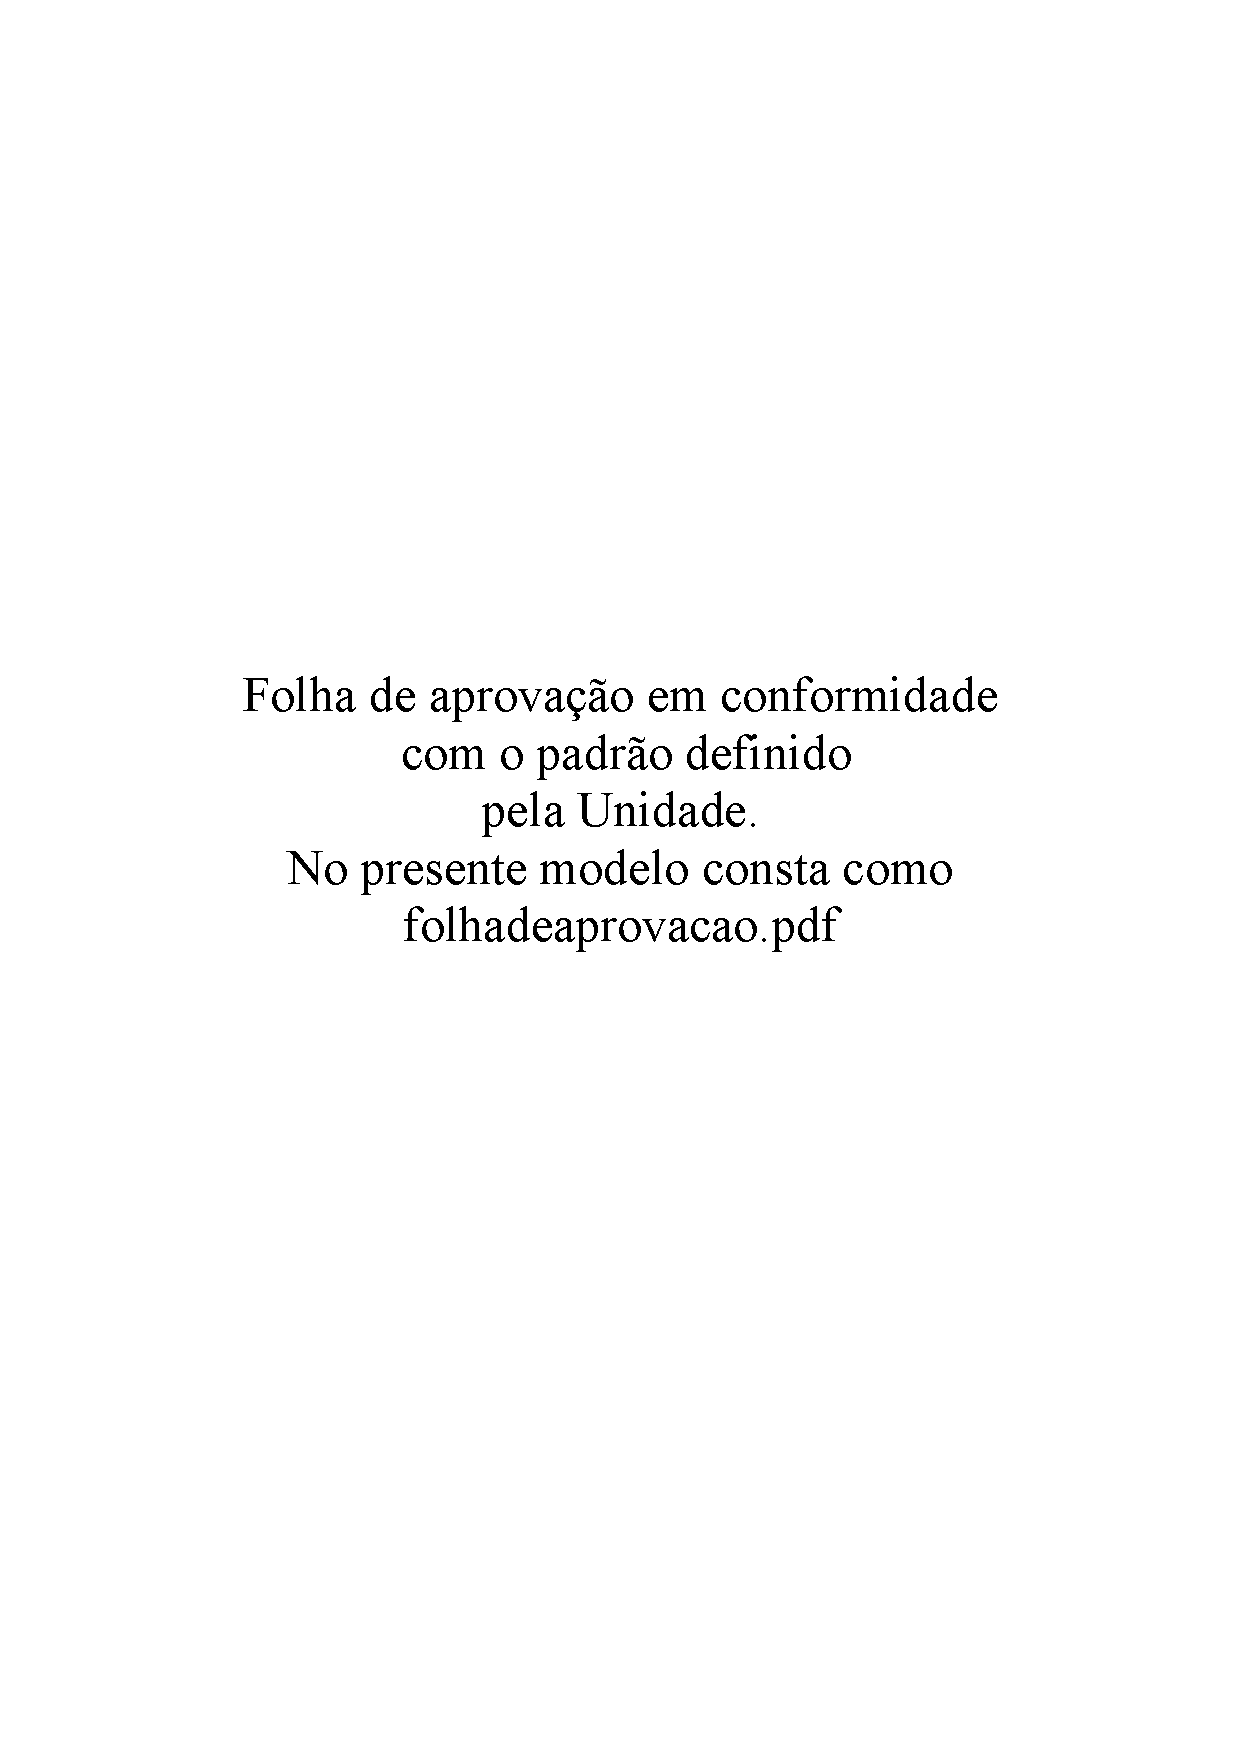
\includepdf{USPSC-TA-PreTextual/USPSC-folhadeaprovacao.pdf}
% Alternativa para a Folha de Aprovação:
% Se for a sua opção elaborar uma folha de aprovação, insira uma % antes do comando acima que inclui o arquivo folhadeaprovacao.pdf,
% tire o % do comando abaixo e altere o arquivo folhadeaprovacao.tex conforme suas necessidades
%\include{folhadeaprovacao}
%
\includepdf{USPSC-TA-PreTextual/USPSC-PaginaEmBranco.pdf}

% ---
% Dedicatória
% ---
%%% USPSC-Dedicatoria.tex
\begin{dedicatoria}
   \vspace*{\fill}
   \centering
   \noindent
   \textit{ Este trabalho é dedicado aos alunos da USP, como uma contribuição\\
  das Bibliotecas do Campus USP de São Carlos para o desenvolvimento\\
	e disseminação da pesquisa científica da Universidade.} \vspace*{\fill}
\end{dedicatoria}
% ---
% ---

% ---
% Agradecimentos
% ---
%%% USPSC-Agradecimentos.tex
\begin{agradecimentos}
	Primeira frase do agradecimento ....
	
	Segunda frase ....
	
	Outras frases ....
	
	Última frase ....
	
\end{agradecimentos}
% ---
% ---

% ---
% Epígrafe
% ---
%%% USPSC-Epigrafe.tex
\begin{epigrafe}
    \vspace*{\fill}
	\begin{flushright}
		\textit{"En remontant chez moi pour y passer la soirée à travailler de mon mieux, je me disais que le monde n'est pas construit pour l'équilibre. Le monde est désordre. L'équilibre n'est pas la règle, c'est l'exception."\\
		G.Duhamel, Maitres, 1937}
	\end{flushright}
\end{epigrafe}
% ---
% ---

% A T E N Ç Ã O
% Se o idioma do texto for em inglês, o abstract deve preceder o resumo
% resumo em português
%
% Resumo
% ---
%% USPSC-Resumo.tex
\setlength{\absparsep}{18pt} % ajusta o espaçamento dos parágrafos do resumo		
\begin{resumo}
	\begin{flushleft} 
			\setlength{\absparsep}{0pt} % ajusta o espaçamento da referência	
			\SingleSpacing 
			\imprimirautorabr~~\textbf{\imprimirtituloresumo}.	\imprimirdata. \pageref{LastPage}p. 
			%Substitua p. por f. quando utilizar oneside em \documentclass
			%\pageref{LastPage}f.
			\imprimirtipotrabalho~-~\imprimirinstituicao, \imprimirlocal, \imprimirdata. 
 	\end{flushleft}
\OnehalfSpacing 	
		
O estudo do espectro de matrizes aleatórias demonstra aplicabilidade em uma gama diversa de áreas da física, matemática à computação e engenharia. Estaremos interessados em estudar os principais ensembles da Teoria de Matrizes Aleatórias e suas medidas de equilíbrio, entender a analogia com Gases de Coulomb e, com essa ferramenta, realizar simulações que nos permitam calcular médias de funções de interesse. Discutiremos quais métodos são importantes para a simulação do problema de gases de coulomb e quais suas limitações além das impostas pela escalabilidade e singularidades do problema. Mostramos que o método de \textit{Langevin Monte Carlo} tem boa performance, possibilitando a réplica de medidas para modelos em uma dimensão bem descritos e, ainda, em extensões de potencial e dimensão menos exploradas.

 \textbf{Palavras-chave}: Gases de Coulomb. Matrizes Aleatórias. 
\end{resumo}
% ---

% Abstract
% ---
%%% USPSC-Abstract.tex
%\autor{Silva, M. J.}
\begin{resumo}[Abstract]
 \begin{otherlanguage*}{english}
	\begin{flushleft} 
		\setlength{\absparsep}{0pt} % ajusta o espaçamento dos parágrafos do resumo		
 		\SingleSpacing  		\imprimirautorabr~~\textbf{\imprimirtitleabstract}.	\imprimirdata.  \pageref{LastPage}p. 
		%Substitua p. por f. quando utilizar oneside em \documentclass
		%\pageref{LastPage}f.
		\imprimirtipotrabalhoabs~-~\imprimirinstituicao, \imprimirlocal, 	\imprimirdata. 
 	\end{flushleft}
	\OnehalfSpacing 
   This is the english abstract.

   \vspace{\onelineskip}
 
   \noindent 
   \textbf{Keywords}: LaTeX. USPSC class. Thesis. Dissertation. Conclusion course paper. 
 \end{otherlanguage*}
\end{resumo}

% ---

% ---
% inserir lista de figurass
% ---
%\pdfbookmark[0]{\listfigurename}{lof}
%\listoffigures*
%\cleardoublepage
% ---

% ---
% inserir lista de tabelas
% ---
%\pdfbookmark[0]{\listtablename}{lot}
%\listoftables*
%\cleardoublepage
% ---

% ---
% inserir lista de quadros
% ---
%\pdfbookmark[0]{\listofquadroname}{loq}
%\listofquadro*
%\cleardoublepage
% ---

% ---
% inserir lista de abreviaturas e siglas
% ---
%% USPSC-AbreviaturasSiglas.tex
\begin{siglas}
    \item[ABNT] Associação Brasileira de Normas Técnicas
    \item[abnTeX] ABsurdas Normas para TeX
	\item[IBGE] Instituto Brasileiro de Geografia e Estatística
	\item[LaTeX] Lamport TeX
	\item[USP] Universidade de São Paulo
	\item[USPSC] Campus USP de São Carlos
\end{siglas}

% ---

% ---
% inserir lista de símbolos
% ---
%% USPSC-Simbolos.tex
\begin{simbolos}
  \item[$ \Gamma $] Letra grega Gama
  \item[$ \Lambda $] Lambda
  \item[$ \zeta $] Letra grega minúscula zeta
  \item[$ \in $] Pertence
\end{simbolos}
% ---
% ---
% inserir o sumario
% ---
\pdfbookmark[0]{\contentsname}{toc}
\tableofcontents*
\cleardoublepage
% ---
% ----------------------------------------------------------
% ELEMENTOS TEXTUAIS
% ----------------------------------------------------------
\textual
% Os capítulos são inseridos como arquivos externos 

% Capítulo 1 - Introdução

% ---
% Capítulo 2
% ---

%\chapter[Introdução]{Introdução}
\label{Introdução}

Sólitons topológicos desempenham papel fundamental no estudo de fenomênos não lineares em diversas áreas da física, eles aparecem em uma variedade de teorias, como \textit{kinks} em $(1+1)$ dimensões, vórtices em $(2+1)$ dimensões, monopolos magnéticos e \textit{Skyrmions} em $(3+1)$ dimensões e \textit{Instantons} em quatro dimensões euclidianas. Os sólitons topológicos são relevantes para muitos fenômenos não lineares na física de altas energias, matéria condensada e na ciência em geral.

Dentre os sólitons topológicos existe uma classe especial, os chamados sólitons auto-duais. Eles são soluções clássicas das equações de auto-dualidade, que são equações de primeira ordem que implicam nas equações de Euler-Lagrange da teoria. Além disso, em cada setor topológico, isto é, o conjunto das soluções que possuem a mesma carga topológica associada, existe um limite inferior da energia estática, ou ação Euclidiana, e os sóltions auto-duais saturam esse limite. Portanto, os sólitons auto-duais são muito estáveis.

A razão pela qual se realiza apenas uma integração para construir os sólitons auto-duais, ao invés de duas para o caso de sóltions topológicos usuais, não está ligada a conservação de uma quantidade dinamicamente. Em todos os casos que a auto-dualidade funciona, a carga topológica relevante admite uma representação integral, ou seja, existe uma densidade de carga topológica. A invariância da carga sobre qualquer variação suave (homotópica) dos campos leva a identidades, em forma de equações diferenciais de segunda ordem, que são satisfeitas por qualquer configuração regular dos campos, não necessariamente solução da teoria. Entretanto, com a imposição das equações de auto-dualidade essas identidades se tornam as equações de Euler-Lagrange da teoria.

Utilizando o conceito de auto-dualidade generalizada se pode criar, com uma carga topológica, uma grande classe de teorias de campo contendo setores auto-duais \cite{lafBPS}. Em $(1+1)$ dimensões foi possível criar teorias de campo, com qualquer número de campos escalares, contendo sólitons topológicos, generalizando o processo conhecido para teorias com somente um campo escalar, como o modelo de \textit{sine-Gordon} e $\lambda \phi^4$ \cite{laf(1+1)}.

Nesse trabalho, serão revisados os recentes desenvolvimentos e aplicações do conceito de auto-dualidade generalizada proposto em \cite{lafBPS}, de uma forma simples e concisa.\footnote{Será utilizada a convenção de soma em índices repetidos durante todo trabalho.}

%\chapter[Autodualidade generalizada]{Autodualidade generalizada}
\label{autodulidade generalizada}

Considere uma teoria de campos que possui uma carga topológica que admite representação integral da forma
\begin{equation}
    \centering
    \mathcal{Q} = \dfrac{1}{2} \int d^{d}x \left [ \mathcal{A}_\alpha \ \tilde{\mathcal{A}}_\alpha^* + \mathcal{A}_\alpha^* \ \tilde{\mathcal{A}}_\alpha \right],
    \label{cargatop}
\end{equation}
onde $\mathcal{A}_\alpha$ e $\tilde{\mathcal{A}}_\alpha$ são funcionais somente dos campos da teoria e das suas primeiras derivadas, onde $*$ se refere somente a conjugado e não transposto conjugado, $\alpha$ se refere a qualquer grupo de índices. O fato de $\mathcal{Q}$ ser topológico significa que ele é invariante por qualquer variação homotópica\footnote{Ou suave.} dos campos. Os campos serão representados por $\chi_\kappa$; eles podem ser escalares, vetoriais ou campos espinores, e o índice $\kappa$ segue a mesma lógica do índice $\alpha$ anterior. Os campos $\chi_\kappa$ serão considerados reais, ou seja, caso existam campos complexos $\chi_\kappa$ assume a parte real e imaginária desses campos.

A invariância de $\mathcal{Q}$ sobre variações suaves dos campos leva à identidade
\begin{equation}
\begin{split}
    \delta\mathcal{Q} = 0 \ \rightarrow \ \ \ &\fdv{\mathcal{A}_\alpha}{\chi_\kappa}\tilde{\mathcal{A}}_\alpha^* - \partial_\mu \left(\fdv{\mathcal{A}_\alpha}{\partial_\mu\chi_\kappa}\tilde{\mathcal{A}}_\alpha^* \right) + \mathcal{A}_\alpha\fdv{\tilde{\mathcal{A}}_\alpha^*}{\chi_\kappa} - \partial_\mu \left( \mathcal{A}_\alpha\fdv{\tilde{\mathcal{A}}_\alpha^*}{\partial_\mu\chi_\kappa} \right) +\\
    & \fdv{\mathcal{A}_\alpha^*}{\chi_\kappa}\tilde{\mathcal{A}}_\alpha - \partial_\mu \left(\fdv{\mathcal{A}_\alpha^*}{\partial_\mu\chi_\kappa}\tilde{\mathcal{A}}_\alpha \right) + \mathcal{A}_\alpha^*\fdv{\tilde{\mathcal{A}}_\alpha}{\chi_\kappa} - \partial_\mu \left( \mathcal{A}_\alpha^*\fdv{\tilde{\mathcal{A}}_\alpha}{\partial_\mu\chi_\kappa} \right) = 0.
\end{split}
\label{identQ}
\end{equation}

Impondo as equações, de primeira ordem, de auto-dualidade nos campos
\begin{equation}
    \mathcal{A}_\alpha = \pm\tilde{\mathcal{A}}_\alpha \ ,  
    \label{bps}
\end{equation}

junto com a identidade (\ref{identQ}), temos as equações
\begin{equation}
\begin{split}
    &\fdv{\mathcal{A}_\alpha}{\chi_\kappa}{\mathcal{A}}_\alpha^* - \partial_\mu \left(\fdv{\mathcal{A}_\alpha}{\partial_\mu\chi_\kappa}{\mathcal{A}}_\alpha^* \right) + \mathcal{A}_\alpha\fdv{{\mathcal{A}}_\alpha^*}{\chi_\kappa} - \partial_\mu \left( \mathcal{A}_\alpha\fdv{{\mathcal{A}}_\alpha^*}{\partial_\mu\chi_\kappa} \right) +\\
    & \fdv{\tilde{\mathcal{A}}_\alpha^*}{\chi_\kappa}\tilde{\mathcal{A}}_\alpha - \partial_\mu \left(\fdv{\tilde{\mathcal{A}}_\alpha^*}{\partial_\mu\chi_\kappa}\tilde{\mathcal{A}}_\alpha \right) + \tilde{\mathcal{A}}_\alpha^*\fdv{\tilde{\mathcal{A}}_\alpha}{\chi_\kappa} - \partial_\mu \left( \tilde{\mathcal{A}}_\alpha^*\fdv{\tilde{\mathcal{A}}_\alpha}{\partial_\mu\chi_\kappa} \right) = 0.
\end{split}
\label{ELident}
\end{equation}

Note que (\ref{ELident}) são as equações de Euler-Lagrange associadas ao funcional
\begin{equation}
    E = \dfrac{1}{2}\int d^d x \left[\mathcal{A}_\alpha \mathcal{A}_\alpha^* + \tilde{\mathcal{A}}_\alpha \tilde{\mathcal{A}}_\alpha^* \right].
    \label{energia}
\end{equation}

Portanto, equações diferenciais de primeira ordem, em conjunto com identidades topológicas de segunda ordem, implicam as equações de Euler-Lagrange de segunda ordem. Além disso, se $E$ for positivo definido, então as soluções auto-duais saturam um limite inferior na energia da seguinte forma. De (\ref{bps}): $\mathcal{A}^2_\alpha = \tilde{\mathcal{A}}^2_\alpha = \pm\mathcal{A}_\alpha\tilde{\mathcal{A}}_\alpha$, (\ref{bps}) também implica $\mathcal{A}_\alpha\tilde{\mathcal{A}}_\alpha^* = \mathcal{A}^*_\alpha\tilde{\mathcal{A}}_\alpha$. Dessa forma, se $\mathcal{A}_\alpha\mathcal{A}^*_\alpha \geq 0$, e consequentemente $\tilde{\mathcal{A}}_\alpha\tilde{\mathcal{A}}^{*}_{\alpha} \geq 0$:
\begin{equation}
\begin{split}
    \mathcal{A}_\alpha = \tilde{\mathcal{A}}_\alpha \ \ \ &\rightarrow \ \ \ \mathcal{Q} = \int d^d x  \ \mathcal{A}_\alpha\mathcal{A}_\alpha^*\\
    \mathcal{A}_\alpha = -\tilde{\mathcal{A}}_\alpha \ \ \ &\rightarrow \ \ \ \mathcal{Q} = -\int d^dx \ \mathcal{A}_\alpha\mathcal{A}^*_\alpha.
\end{split}
\end{equation}

Dessa forma, é possível reescrever o funcional de energia (\ref{energia}) como
\begin{equation}
    E = \dfrac{1}{2} \int d^dx \left[ \mathcal{A}_\alpha \mp \tilde{\mathcal{A}}_\alpha \right] \left[\mathcal{A}^*_\alpha \mp \tilde{\mathcal{A}}_\alpha^* \right] \pm \dfrac{1}{2} \int d^dx \left[\mathcal{A}_\alpha \tilde{\mathcal{A}}_\alpha^* + \mathcal{A}^*_\alpha \tilde{\mathcal{A}}_\alpha\right] \geq \abs{\mathcal{Q}} \ ,
\end{equation}

onde, para soluções auto-duais, vale a igualdade da relação
\begin{equation}
    E = \int d^dx \ \mathcal{A}_\alpha\mathcal{A}^*_\alpha = \int d^dx \ \tilde{\mathcal{A}}_\alpha\tilde{\mathcal{A}}_\alpha^* = \abs{\mathcal{Q}} \ .
\end{equation}

A forma de separar o integrando de $\mathcal{Q}$ em (\ref{cargatop}) é bastante arbitrária, mas feita essa escolha ainda é possível realizar uma transformação simples da seguinte forma:
\begin{equation}
    \mathcal{A}_\alpha \rightarrow \mathcal{A}_\alpha' = \mathcal{A}_\beta k_{\beta\alpha} \ ; \ \ \ \ \tilde{\mathcal{A}}^*_\alpha \rightarrow (\tilde{\mathcal{A}}'_\alpha)^* = k^{-1}_{\alpha\beta} \tilde{\mathcal{A}_\beta^*} \ .
    \label{trasnf_geral}
\end{equation}

Essa transformação não muda a forma da carga topológica, portanto $\mathcal{Q}$ continua invariante por transformações homotópicas dos campos. Logo, o mesmo desenvolvimento anterior para os funcionais $\mathcal{A}_\alpha$ e $\tilde{\mathcal{A}}_\alpha$ pode ser repetido para os funcionais transformados $\mathcal{A}'_\alpha$ e $\tilde{\mathcal{A}}'_\alpha$. Assim, as novas equações de auto-dualidade são
\begin{equation}
    \mathcal{A}_\beta k_{\beta\alpha} = \pm (k^{-1}_{\alpha\beta})^*\tilde{\mathcal{A}}_\beta \ \ \ \rightarrow \ \ \ \mathcal{A}_\beta h_{\beta\alpha} = \pm \tilde{\mathcal{A}}_\alpha \ ,
    \label{bps2}
\end{equation}
em que foi definida a matriz inversível e hermitiana:
\begin{equation}
    h \equiv kk^{\dag} \ .
\end{equation}

Junto com as identidades transformadas (\ref{identQ}), as novas equações de auto-dualidade (\ref{bps2}) implicam as equações de Euler-Lagrange do funcional
\begin{equation}
    E' = \dfrac{1}{2} \int d^dx \left[\mathcal{A}_\alpha h_{\alpha\beta} \mathcal{A}^*_\beta + \tilde{\mathcal{A}_\alpha}h^{-1}_{\alpha\beta} \tilde{\mathcal{A}}^*_\beta\right]
    \label{energia2} \ .
\end{equation}

Note que a matriz $h$ pode introduzir novos campos na teoria sem mudar a carga topológica.

Além disso, de (\ref{bps2}): $\mathcal{A}_\alpha h_{\alpha\beta} \mathcal{A}^*_\beta = \tilde{\mathcal{A}}_\alpha h^{-1}_{\alpha\beta}\tilde{\mathcal{A}}^*_\beta = \pm \mathcal{A}_\alpha\tilde{\mathcal{A}}^*_\alpha = \pm \mathcal{A}^*_\alpha\tilde{\mathcal{A}}_\alpha$. Portanto, se $\mathcal{A}_\beta h_{\beta\alpha}\mathcal{A}^*_\alpha \geq 0$, e consequentemente $\tilde{\mathcal{A}}_\alpha h^{-1}_{\alpha\beta}\tilde{\mathcal{A}}_\beta^* \geq 0$, o limite inferior na energia ($E'$ nesse caso) segue da mesma forma que anteriormente
\begin{equation}
\begin{split}
    E' &= \dfrac{1}{2} \int d^dx \left[\mathcal{A}_\beta k_{\beta\alpha} \mp (k^{-1}_{\alpha\beta})^*\tilde{A}_\beta \right] \left[\mathcal{A}_\gamma^*k^*_{\gamma\alpha} \mp k^{-1}_{\alpha\gamma}\mathcal{A}^*_\gamma \right] \\[0.2cm]
    &\pm \dfrac{1}{2} \int d^dx \left[\mathcal{A}_\alpha\tilde{\mathcal{A}}^*_\alpha + \mathcal{A}^*_\alpha \tilde{\mathcal{A}}_\alpha \right] \geq \abs{\mathcal{Q}} \ .
\end{split}
\end{equation}

A seguir, serão examinadas algumas teorias em que são aplicadas as ideias discutidas nessa seção.

%\chapter[\textit{Kinks} com vários campos em (1+1) dimensões]{\textit{Kinks} com vários campos em (1+1) dimensões}
\label{(1+1) dimensões}

Setores auto-duais para teorias em $(1+1)$ dimensões, contendo somente um campo escalar, como modelos de \textit{sine-Gordon} e $\lambda\phi^4$, são conhecidos há bastante tempo. A aplicação das ideias discutidas nas seções anteriores levou a construção de setores auto-duais em teorias em $(1+1)$ dimensões com qualquer número de campos escalares \cite{laf(1+1)}. Nesta seção serão considerados campos escalares reais. A carga topológica nesse caso é
\begin{equation}
    \mathcal{Q} = \int^{\infty}_{-\infty} \dd x \dv{U}{x} = \int^{\infty}_{-\infty}\dd x \fdv{U}{\varphi_a}\dv{\varphi_a}{x} = U(\varphi_a(x=\infty)) - U(\varphi_a(x=-\infty)) \ ,
\end{equation}
em que $U$ é um funcional real arbitrário dos campos $\varphi_a$, $a = 1,2,...,r$, mas não de suas derivadas.\footnote{Isso será importante para que a carga topológica não seja função de derivadas de mais do que primeira ordem dos campos.} A equação acima está na mesma forma de (\ref{cargatop}), assim é possível realizar as identificações
\begin{equation}
    \mathcal{A}_\alpha \equiv k_{\alpha\beta}\dv{\varphi_\beta}{x} \ ; \ \ \ \ \ \ \Tilde{\mathcal{A}}_\alpha \equiv \fdv{U}{\varphi_\beta}k^{-1}_{\beta\alpha} \ ,
\end{equation}
onde os funcionais $\mathcal{A}_\alpha$, $\Tilde{\mathcal{A}}_\alpha$ e $k$ são reais, e a matriz $k$ também é inversível e arbitrária. De acordo com (\ref{bps2}), as equações auto-duais são
\begin{equation}
    \eta_{ab}\dv{\varphi_b}{x} = \pm\fdv{U}{\varphi_a} \ ; \ \ \ \ \ \ \ \ \eta = k^{T}k \ .
    \label{bps1d}
\end{equation}

Então, $\eta$ é uma matriz simétrica e inversível. Seguindo (\ref{energia2}), a energia estática da nossa teoria se torna
\begin{equation}
    E = \int^{\infty}_{-\infty} \dd x \left[\dfrac{1}{2}\eta_{ab}\dv{\varphi_a}{x}\dv{\varphi_b}{x} + V \right] \ ,
    \label{funcE}
\end{equation}
onde a forma do potencial é
\begin{equation}
    V = \dfrac{1}{2} \ \eta^{-1}_{ab} \ \fdv{U}{\varphi_a}\fdv{U}{\varphi_b} \ .
    \label{potencial}
\end{equation}

Portanto, dos argumentos da seção anterior, segue que as soluções de (\ref{bps1d}) são também soluções das equações de Euler-lagrange do funcional (\ref{funcE}), onde a quantidade $U$ desempenha o papel de um pré-potencial. Note que, dado a escolha de um pré-potencial $U$, é possível determinar o potencial $V$ e também uma teoria de campos escalares com um setor auto-dual. Entretanto, dado um potencial, não é trivial encontrar o pré-potencial $U$; tendo isso em vista, será discutida a construção de teorias auto-duais por meio da escolha do pré-potencial. Nesse sentido, a análise será restringida para casos em que os campos escalares $\varphi_a$, o pré-potencial $U$ e a matriz $\eta$ sejam reais. Além disso, é imposto que o funcional $E$ (\ref{funcE}) seja positivo definido, dessa forma os autovalores de $\eta$ também devem ser positivos.

Para que as soluções auto-duais de (\ref{bps1d}) tenham energia finita, é necessário que a densidade de energia em (\ref{funcE}) desapareça para infinitos espaciais quando evaluado nessas soluções, logo é necessário que
\begin{equation}
    \dv{\varphi_a}{x} \rightarrow 0 \ ; \ \ \ \ \ \ \fdv{U}{\varphi_a} \rightarrow 0 \ ; \ \ \ \ \ \ \text{com} \ \ \ \ \ \ x \rightarrow \pm \infty.
    \label{phi_U_zero}
\end{equation}

Portanto, as equações de auto-dualidade (\ref{bps1d}) devem possuir soluções constantes de vácuo $\varphi_a^{(vac)}$ que sejam zeros para todas derivadas do pré-potencial, ou seja,
\begin{equation}
    \eval{\fdv{U}{\varphi_c}}_{\varphi_a = \varphi_a^{(vac)}} = 0.
    \label{dU_zero}
\end{equation}

De (\ref{potencial}), essas soluções de vácuo também são zeros do potencial $V$ e de suas primeiras primeiras derivadas, ou seja,
\begin{equation}
    V\left(\varphi_a^{(vac)}\right) = 0 \ ; \qquad \qquad \eval{\fdv{V}{\varphi_c}}_{\varphi_a = \varphi_a^{(vac)}} = 0 \ .
\end{equation}

Ademais, é desejável que as teorias contruídas tenham diversas soluções tipo sóliton, e que tenham um sistema de vácuos tão degenerados quanto possível para manter as estruturas topológicas não triviais de $\mathcal{Q}$. Existem diversas formas de obter esse sistema de vácuos; nesse trabalho, será adotado o mesmo procedimento que em \cite{laf(1+1)}, baseado na teoria de grupos. Não será discutido o procedimento de criação dos pré-potenciais; para detalhes, consultar \cite{laf(1+1)}.

\section{Interpretação mecânica de soluções auto-duais.}

Tendo como base os desenvolvimentos em (\ref{phi_U_zero}) e (\ref{dU_zero}), soluções da equação de auto-dualidade (\ref{bps1d}) com energia finita devem tender a soluções constantes de vácuo quando $x\rightarrow \pm \infty$. Assim, cada uma dessas soluções conecta dois vácuos da teoria. Para desenvolver uma visualização geométrica dessas soluções, serão reescritas as equações de auto-dualidade da seguinte forma:
\begin{equation}
    \Vec{v} = \pm \Vec{\nabla}_{\eta}U \ ; \quad \quad \quad \text{com} \quad \quad \quad (\Vec{v})_a = \dv{\varphi_a}{x} \ ; \qquad \left(\Vec{\nabla}_{\eta}U \right)_a = \eta^{-1}_{ab} \fdv{U}{\varphi_b} \ .
\end{equation}

Dado o potencial $U$ e a métrica $\eta$, que é real, constante e positiva, $\Vec{\nabla}_\eta U$ define curvas no espaço dos campos ($\varphi_1, \varphi_2, \ ... \ , \varphi_r$),\footnote{O índice utilizado ($r$) a príncipio não possui qualquer significado, mas o uso se deu devido ao conceito de \textit{rank} de uma álgebra de Lie. No caso das construções utilizando teoria de grupos: $r = \textit{rank} \ (\mathcal{G}).$} fazendo o papel de vetor tangente a essas curvas. Essas curvas não se intersectam; para manter $\Vec{\nabla}_\eta U$ bem definido em qualquer ponto do espaço dos campos, no máximo elas podem se tocar tangencialmente ou se encontrar em pontos em que $\Vec{\nabla}_\eta U$ zera. A equação de auto-dualidade (\ref{bps1d}) é uma equação diferencial de primeira ordem, logo uma solução é determinada pelo valor dos campos $\varphi_a$ em um ponto $x = x_0$. 

A visão geométrica é a de uma partícula viajando no espaço dos $\varphi_a$ com \textit{x-velocidade} $\Vec{v}$ e com a coordenada espacial $x$ desempenhando o papel do tempo. Portanto, o problema de resolver a equação de auto-dualidade se reduz ao de construir curvas no espaço dos campos determinadas por $\Vec{\nabla}_\eta U$. As soluções de energia finita correponderão às curvas que começam e terminam nos extremos do pré-potencial $U$, ou seja, nos pontos em que $\Vec{\nabla}_\eta U = 0$.

Considere agora uma curva $\gamma$ no espaço dos campos, parametrizada por $x$, ou seja, $\varphi_a(x)$, que seja solução das equações de auto-dualidade (\ref{bps1d}). Associada a essa curva é definida a quantidade
\begin{equation}
    \Tilde{\mathcal{Q}}(\gamma) = \int_{\gamma}\dd x \ \Vec{v}\cdot\Vec{\nabla}U = \int_{\gamma}\dd x \ \dv{\varphi_a}{x}\fdv{U}{\varphi_a} = U(x_f) - U(x_i),
    \label{Qdiff}
\end{equation}
em que $x_f$ e $x_i$ são os pontos final e inicial, respectivamente, da curva $\gamma$. Perceba que o vetor tangente à curva é $\Vec{\nabla}_\eta U$ e não $\Vec{\nabla}U$, uma vez que a curva é solução das equações (\ref{bps1d}). Utilizando as equações de auto-dualiadade é possível reescrever a equação (\ref{Qdiff}) da seguinte forma:
\begin{equation}
    \Tilde{\mathcal{Q}}(\gamma) = \pm \int_{\gamma} \dd x \ \eta_{ab}\dv{\varphi_a}{x}\dv{\varphi_b}{x} = \pm \int_{\gamma} \dd x \ \omega_a \left(\dv{\tilde{\varphi_a}}{x} \right)^2,
\end{equation}
em que a matriz $\eta$ foi diagonalizada, ou seja, 
\begin{equation}
    \eta = \Lambda^{T}\eta^D\Lambda \ ; \qquad \quad \Lambda^T\Lambda = \mathbb{1} \ ; \quad\qquad \eta_{ab}^D = \omega_a\delta_{ab} \ ; \quad \qquad \omega_a > 0 \ ,
\end{equation}
onde foi assumido que todos autovalores de $\eta$ são positivos, e foi definido $\Tilde{\varphi_a} = \Lambda_{ab}\varphi_b$. Mantendo $\eta$ como positiva definida, a quantidade $\Tilde{\mathcal{Q}}(\gamma)$ só pode assumir o valor zero se os campos forem constantes por toda curva, ou seja, a curva teria que se reduzir a um ponto. Logo, as soluções das equações de auto-dualidade (\ref{bps1d}) não podem começar e acabar em pontos no espaço dos campos em que o pré-potencial $U$ possui o mesmo valor. Além disso, conforme alguém \textit{anda} pela curva a diferença do valor do pré-potencial de um particular ponto e do ponto inicial sempre aumenta em módulo. Portanto, a curva, que é solução das equações (\ref{bps1d}), sempre \textit{escala} o pré-potencial $U$, para cima ou para baixo dependendo do sinal tomado na equação (\ref{bps1d}), sem nunca retornar a uma altitude já atingida. 

\section{Exemplo -- $SU(3)$}

Nesta seção será apresentado um exemplo concreto dos conceitos discutidos nas seções (\ref{autodulidade generalizada}) e (\ref{(1+1) dimensões}). No exemplo que segue, a matriz $\eta$ será constante\footnote{Isto é, não irá depender dos campos $\varphi_a$ da teoria ou de outros campos externos.}, real e positiva definida. Mesmo com essas restrições ainda é possível construir teorias interessantes.

O \textit{rank} de $SU(3)$ é dois, portanto a teoria possuirá dois campos $\varphi_1$ e $\varphi_2$. A matriz $\eta$ é escolhida tal que\footnote{Note que $ \eta|_{\lambda = 1} = K$, com $K$ sendo a matriz de Cartan de $SU(3)$. \cite{lafGRUPOS}}
\begin{equation}
    \eta = \mqty(2 & -\lambda \\ -\lambda & 2) \ ; \qquad\qquad \eta^{-1} = \dfrac{1}{4-\lambda^2} \mqty(2 & \lambda \\ \lambda & 2) \ ,
\end{equation}
onde foi introduzido o parâmetro real $\lambda$. Os autovalores de $\eta$ são $2\pm \lambda$, portanto $\lambda$ deve se manter no intervalo $2 < \lambda < -2$, para manter $\eta$ positiva definida e inversível. Por meio de um procedimento utilizando teoria de grupos\footnote{A construção se baseia nos pesos das representações da algebra. Para mais detalhes consultar \cite{laf(1+1)}.}, é obtido o pré-potencial
\begin{equation}
    U = \gamma_1 \cos\qty(\varphi_1) + \gamma_2 \cos\qty(\varphi_2) + \gamma_3 \cos\qty(\varphi_1 - \varphi_2) \ ,
    \label{U_SU3}
\end{equation}
em que $\gamma_1$, $\gamma_2$ e $\gamma_3$ são constantes arbitrárias.

A energia estática (\ref{funcE}) se torna
\begin{equation}
    E = \int^{\infty}_{-\infty} \dd x \ \qty[\qty(\partial_x \varphi_1)^2 + \qty(\partial_x \varphi_2)^2 - \lambda\partial_x\varphi_1\partial_x\varphi_2 + V\qty(\varphi_1, \varphi_2)] \ ,
\end{equation}
onde o potencial (\ref{potencial}) é dado por
\begin{equation}
\begin{aligned}
 	V &= \dfrac{1}{\lambda^2 - 4}[-\gamma_1^2\sin^2(\varphi_1) + \gamma_1\sin(\varphi_1)\qty(\gamma_3\qty(\lambda -2)\sin (\varphi_1 - \varphi_2) - \gamma_2\lambda\sin(\varphi_2)) \\
	   & - \gamma_2^2\sin^2(\varphi_2) - \gamma_2\gamma_3\qty(\lambda-2)\sin(\varphi_2)\sin(\varphi_1-\varphi_2)+\gamma_3^2\qty(\lambda -2)\sin^2(\varphi_1-\varphi_2)] \ .
    \label{V_SU3}
\end{aligned}
\end{equation}

As equações de auto-dualidade (\ref{bps1d}) são da forma
\begin{equation}
\begin{aligned}
    &\partial_x\varphi_1 = \pm \dfrac{\qty[2\gamma_1\sin(\varphi_1) + \lambda\gamma_2\sin(\varphi_2) - \gamma_3\qty(\lambda-2)\sin(\varphi_1-\varphi_2)]}{\lambda^2 - 4}, \\
    &\partial_x\varphi_2 = \pm \dfrac{\qty[2\gamma_2\sin(\varphi_2) + \lambda\gamma_1\sin(\varphi_1) + \gamma_3\qty(\lambda-2)\sin(\varphi_1-\varphi_2)]}{\lambda^2 - 4}.
\end{aligned}
\end{equation}

Os vácuos são determinados pelas condições (\ref{dU_zero}), que implicam
\begin{equation}
    \gamma_1\sin\qty(\varphi_1^{(vac)})=-\gamma_3\sin\qty(\varphi_1^{(vac)}-\varphi_2^{(vac)}) = - \gamma_2 \sin\qty(\varphi_2^{(vac)}).
\end{equation}

Certamente, a equação acima é satisfeita se
\begin{equation}
    \varphi_a^{(vac)} = n_a \pi \ , \qquad\qquad n_a \in \mathbb{Z}, \qquad\qquad a=1,2 \ ,
    \label{vac_normal}
\end{equation}
para qualquer valor para os coeficientes $\gamma$. Entretanto, existem outros tipos de vácuo que dependem do valor escolhido para cada $\gamma$, como 
\begin{equation}
\begin{aligned}
    & \qty(\varphi_1^{(vac)}, \varphi_2^{(vac)}) = \qty(\dfrac{2\pi}{3} + 2\pi \, n_1 \, , \ \dfrac{4\pi}{3} + 2\pi \, n_2) \ ; \qquad \qquad \gamma_1=\gamma_2=\gamma_3 = 1, \\
    & \qty(\varphi_1^{(vac)}, \varphi_2^{(vac)}) = \qty(\dfrac{4\pi}{3} + 2\pi \, n_1 \, , \ \dfrac{2\pi}{3} + 2\pi \, n_2) \ ; \qquad\qquad n_1 \, , \, n_2 \in \mathbb{Z} \ .
    \label{vac_especial}
\end{aligned}
\end{equation}


\begin{figure}[ht] 
  \begin{subfigure}[b]{0.5\linewidth}
    \centering
    \includegraphics[width=0.95\linewidth]{USPSC-img/U_SU(3)_(3D).png} 
    \caption{} 
    \label{fig7:a} 
    \vspace{4ex}
  \end{subfigure}%% 
  \begin{subfigure}[b]{0.5\linewidth}
    \centering
    \includegraphics[width=0.95\linewidth]{USPSC-img/V_SU(3)_Lambda=1.0_(3D).png} 
    \caption{} 
    \label{fig7:b} 
    \vspace{4ex}
  \end{subfigure} 
  \begin{subfigure}[b]{0.5\linewidth}
    \centering
    \includegraphics[width=0.95\linewidth]{USPSC-img/U_SU(3)_(2D).png} 
    \caption{} 
    \label{fig7:c} 
  \end{subfigure}%%
  \begin{subfigure}[b]{0.5\linewidth}
    \centering
    \includegraphics[width=0.95\linewidth]{USPSC-img/V_SU(3)_Lambda=1.0_(2D).png} 
    \caption{} 
    \label{fig7:d} 
  \end{subfigure} 
  \caption{(a) e (c) são representações do pré-potencial (\ref{U_SU3}), e (b) e (c) do potencial (\ref{V_SU3}). Os vácuos do tipo (\ref{vac_normal}) são os pontos pretos, enquanto os do tipo (\ref{vac_especial}) são denotados por quadrados em branco. As linhas representam o fluxo de $\grad U$ e $\grad V$, em que $\grad = \qty(\partial_{\varphi_1}, \partial_{\varphi_2})$. Nos gráficos, foi utilizado $\lambda = 1$ e $\gamma_1 = \gamma_2 = \gamma_3 = 1$.}
  \label{fig7} 
\end{figure}

% ---
%\chapter[\textit{Lumps} em $(2+1)$ dimensões]{\textit{Lumps} em $(2+1)$ dimensões}
\label{Lumps (2+1)}

Como um exemplo de uma teoria com um setor auto-dual, será considerado o modelo $\mathbb{CP}^{N-1}$ em (2+1) dimensões. $\mathbb{CP}^{N-1}$ é o espaço projetivo complexo de ($N-1$) dimensões, ou seja, o espaço de todas as classes equivalentes de vetores complexos $z = \left(z_1 \ , \ z_2 \ , \ ... \ , \ z_N\right)$, tal que dois vetores $z$ e $z'$ são equivalentes se $z' = \lambda z$, sendo $\lambda$ um número complexo \cite{sigmamodelinst, lowsigma}. Serão considerados os representantes dessas classes como os vetores unitários
\begin{equation}
    z = (z_1,z_2,...,z_N) \ ; \qquad \qquad \qquad z^{*}_a z_a = 1 \ .
\end{equation}

$\mathbb{CP}^{N-1}$ é isomórfico a $SU(N)/SU(N-1) \otimes U(1)$. De fato, o grupo $SU(N)$ age transitivamente nos vetores $z$ por meio da sua representação definidora $N-\text{dimensional}$. Como essa representação é unitária, sua ação preserva o módulo dos vetores $z$, e um dado vetor é mantido invariante por matrizes $(N-1)\times(N-1)$ unitárias, ou seja, o subgrupo $U(N-1) = SU(N-1)\otimes U(1)$.

O segundo grupo de homotopia de $\mathbb{CP}^{N-1}$ é isomórfico aos inteiros sobre adição, ou seja, $\pi_2\left(SU(N)/SU(N-1)\otimes U(1)\right) = \mathbb{Z}$. A carga topológica associada possui uma representação integral da forma
\begin{equation}
    \mathcal{Q} = \dfrac{1}{2\pi}\int \dd^2 x \ \varepsilon_{\mu \nu}\partial_\mu A_\nu \ ,
    \label{Q(2+1)}
\end{equation}
onde
\begin{equation}
    A_\mu = \dfrac{i}{2}\left(z^{\dag}\partial_\mu z - \partial_\mu z^{\dag} z\right) \ .
\end{equation}
A integração em (\ref{Q(2+1)}) é no plano bidimensional $(x_1 , x_2)$, que, identificando o infinito espacial, é isomórfico à $S^2$.\footnote{Superfície da esfera tridimensional.} Sobre a transformação local $z \rightarrow e^{i\alpha}z$, será obtido $A_\mu \rightarrow A_\mu -\partial_\mu \alpha$. Definindo a derivada covariante $D_\mu \equiv \partial_\mu + i A_\mu$, (\ref{Q(2+1)}) pode ser reescrita como
\begin{equation}
    \mathcal{Q} = \dfrac{i}{2\pi} \int \dd^2 x \ \varepsilon_{\mu\nu}\left(D_\mu z \right)^{\dag}\left(D_\nu z\right) = \dfrac{1}{4\pi} \int \dd^2 x \left[\left(D_\mu z \right)^{\dag} i \, \varepsilon_{\mu\nu} \, D_\nu z + \left( i \,  \varepsilon_{\mu\nu} \, D_\nu z\right)^{\dag} D_\mu z \right].
    \label{carga(2)}
\end{equation}
Seguindo (\ref{trasnf_geral}), são definidas as quantidades:
\begin{equation}
    \mathcal{A}^a_\mu = \left( D_\mu z\right)_b k_{ba} \ ; \qquad \qquad \Tilde{\mathcal{A}}_{\mu}^{a} = \left( k^{-1}_{ab} \right)^* i \, \varepsilon_{\mu\nu} \, \left(D_\nu z \right)_b \ , 
\end{equation}
logo a carga (\ref{carga(2)}) pode ser escrita na forma (\ref{cargatop}). De (\ref{bps2}), as equações de auto-dualidade são
\begin{equation}
    \left(D_\mu z\right)_b h_{ba} = \pm \, i \, \varepsilon_{\mu\nu} \left(D_\nu z\right )_a \ .
    \label{bps2d}
\end{equation}
De acordo com (\ref{energia2}), o funcional da energia se torna
\begin{equation}
    E = \dfrac{1}{2} \int \dd^2x \left[\left(D_\mu z\right)_a^* h_{ab} \left(D_\mu z\right)_b + \left(D_\mu z\right)_a^* h^{-1}_{ab} \left(D_\mu z\right)_b  \right] \ .
    \label{E2d}
\end{equation}
Contraindo os dois lados de (\ref{bps2d}) com $\varepsilon_{\rho \mu}$, obtém-se
\begin{equation}
    \left(D_\mu z\right)_a = \pm \, i \, \varepsilon_{\mu\nu} \, \left(D_\nu z\right)_b h_{ba} \ .
    \label{relacao_eps}
\end{equation}
Portanto, (\ref{bps2d}) e (\ref{relacao_eps}) implicam
\begin{equation}
    \left(D_\mu z \right)_b \left(h_{ba} - h^{-1}_{ba} \right) = 0 \qquad \rightarrow \qquad h^2 = \mathbb{1} \ ,
    \label{4.9}
\end{equation}
mas uma matriz hermitiana pode ser diagonalizada por uma transformação unitária, $h = Uh_DU^{\dag}$, com $h_D$ diagonal. Logo
\begin{equation}
    h^2 = \mathbb{1} \qquad \qquad \rightarrow \qquad\qquad h^2_D = \mathbb{1} \ ,
\end{equation}
assim $\lambda_a^2 = 1$. Porém, para a energia $E$ (\ref{E2d}) ser positiva definida, é necessário que todos autovalores de $h$ tenham o mesmo sinal. Então
\begin{equation}
    h = \mathbb{1} \ .
    \label{4.11}
\end{equation}
Nesse caso, (\ref{bps2d}) reduz-se às equações de auto-dualidade para o modelo $\mathbb{CP}^{N-1}$ usual \cite{sigmamodelinst, lowsigma},
\begin{equation}
    \left(D_\mu z\right)_a = \pm \, i \, \varepsilon_{\mu\nu} \left(D_\nu z\right )_a \ ,
    \label{bps2d_2}
\end{equation}
e (\ref{E2d}) à energia usual do modelo $\mathbb{CP}^{N-1}$,
\begin{equation}
    E = \int \dd^2x \left(D_\mu z \right)^{\dag} D_\mu z \ .
\end{equation}

Para construir soluções auto-duais da equação (\ref{bps2d_2}), é conveniente introduzir novos campos complexos $u_a$ como
\begin{equation}
    (u_1^{(j)}, u_2^{(j)}, ... , u_{N-1}^{(j)}, u_N^{(j)}) = \dfrac{1}{z_j}(z_1,z_2,...,z_{N-1},z_N) \ ,
\end{equation}
em que $u_j^{(j)} = 1$, ou seja, as coordenadas são $u_\alpha^{(j)}, \alpha\neq j$. Pode ser escolhida qualquer componente $z_a$ para construir o campo $u_a$; nesse caso, será escolhida a componente $z_N$, logo $u_\alpha , \alpha = 1,...,N-1$ são as coordenadas. Podemos reescrever a equação (\ref{bps2d_2}) em termo das novas coordenadas da seguinte forma: \cite{sigmamodelinst}
\begin{equation}
    \partial_\mu u_\alpha = \pm \, i \, \varepsilon_{\mu\nu} \, \partial_\nu u_\alpha \ ; \qquad \qquad \alpha = 1,2,...,N-1.
\end{equation}

Essas são as equações de Cauchy-Riemann para os campos $u$. De fato, o sinal $(+)$ implica que $u$ é holomórfico, ou seja, $u_\alpha = u_\alpha(\omega)$, e o sinal $(-)$ que $u$ é anti-holomórfico, ou seja, $u_\beta = u_\beta(\omega^*)$, em que $\omega = x_1 + i x_2$.

%\chapter[$(3+1)$ Dimensões e Instantons em $(4+0)$ dimensões]{$(3+1)$ Dimensões e Instantons em $(4+0)$ dimensões}
\label{(3+1) e 4}

\section{Monopolos}

Será considerado o caso da carga magnética topológica definida pela integral no espaço de três dimensões $\mathbb{R}^3$
\begin{equation}
    \mathcal{Q}_M = -\dfrac{1}{2}\int_{\mathbb{R}^3} \dd^3x \, \varepsilon_{ijk} \, \text{Tr}\left(F_{ij}D_k\Phi \right) = \int_{\mathbb{R}^3} \dd^3x \, \text{Tr}\left(B_i D_i \right) \ ,
    \label{Qmonopolo}
\end{equation}
onde $B_i = -\dfrac{1}{2}\, \varepsilon_{ijk}\, F_{jk}$ é o campo magnético não abeliano, $F_{ij} = \partial_iA_j - \partial_j A_i - ie\comm{A_i}{A_j} = F^a_{ij} T_a$ o tensor dos campos, $A_i = A_i^a T_a$ o campo de \textit{gauge}, e $\Phi = \Phi^{a}T_a$ o campo de \textit{Higgs} na representação adjunta de um grupo de Lie simples e compacto, com geradores $T_a \, , \ a = 1,2,...,\text{dim} \, G$. Além disso, $D_i \qty(*) = \partial_i \qty(*) + ie \comm{A_i}{\qty(*)} $ é a derivada covariante na representação adjunta de $G$.

Nesse caso todos os campos são reais. Logo, seguindo (\ref{bps2}) e os resultados em \cite{LafHenBPS}, são introduzidas as quantidades reais
\begin{equation}
    \mathcal{A}_\alpha \equiv B_i^b \, k_{ba} \ ; \qquad \qquad \tilde{\mathcal{A}}_\alpha \equiv k^{-1}_{ab} \qty(D_i\Phi)^b \ ,
\end{equation}
então (\ref{Qmonopolo}) pode ser escrita como (\ref{cargatop}). As equações de auto-dualidade (\ref{bps2}) se tornam
\begin{equation}
    \dfrac{1}{2} \, \varepsilon_{ijk}F_{jk}^b\, h_{ba} = \pm \qty(D_i \Phi)^a \ ; \qquad\qquad\qquad h = k\,k^T \ ,
    \label{bpsmonopolo}
\end{equation}
com $h_{ab}$, $a,b = 1,2,...,\text{dim} \, G$, uma matriz simétrica e inversível de campos escalares. As equações (\ref{bpsmonopolo}) constituem uma generalização das equações \textit{BPS} (\textit{Bogomolny-Prasad-Sommerfield}) \cite{bps_1976, monopolohooft} para monopolos auto-duais. O funcional de energia (\ref{energia2}) se torna \cite{LafHenBPS}
\begin{equation}
    E_{YMH} = \int \dd^3x \, \qty[\dfrac{1}{4}h_{ab}F^{a}_{ij}F^b_{ij} + \dfrac{1}{2}h^{-1}_{ab} \qty(D_i\Phi)^a \qty(D_i\Phi)^b] \ ,
    \label{Emonopolo}
\end{equation}
portanto essa é uma teoria com campos de \textit{gauge} $A_\mu$, campo de Higgs $\Phi$ na representação adjunta do grupo de \textit{gauge}, e campos escalares reais na matriz $h$. A energia (\ref{Emonopolo}) avaliada nas soluções auto-duais de (\ref{bpsmonopolo}) é igual à carga magnética topológica
\begin{equation}
    E_{YMH} = \mathcal{Q}_M \ .
\end{equation}

Para mais detalhes na construção de soluções auto-duais dessa teoria, consultar \cite{LafHenBPS}.

\section{Skyrmions}

Skyrmions são sólitons topológicos soluções de teorias em $(3+1)$ dimensões com o grupo $SU(2)$ como espaço-alvo. Os três campos em $SU(2)$ são interpretados como os três píons $\pi^+, \pi^0$ e $\pi^-$. Essas soluções são interpretadas seguindo a proposta de Skyrme \cite{skyrmeNonLinear, skyrmeMesons}, em que a carga topológica desempenha o papel de número bariônico \cite{TopSol, shnirTop}.

A carga topológica relevante nesse caso é dada pela integral sobre o espaço tridimensional $\mathbb{R}^3$
\begin{equation}
    \mathcal{Q}_B = \dfrac{i}{48\pi^2}\int \dd^3x \, K(U) \, \varepsilon_{ijk} \, \text{Tr}\qty(R_i R_j R_k) \ ,
    \label{QSkyrm}
\end{equation}
com $R_i = i\partial_i U U^{\dag} = R_i^{a}T_a$, $U \ \in \ SU(2)$, e $K(U)$ é um funcional real arbitrário dos campos quirais $U$, mas não de suas derivadas. $K$ pode ser interpretado como uma deformação na métrica do espaço-alvo $SU(2)$. A notação utilizada é tal que $\text{Tr}\qty(T_aT_b) = \delta_{ab}$, com $T_a \, , \ a=1,2,3$ sendo os geradores da álgebra de Lie de $SU(2)$.

Seguindo (\ref{cargatop}), serão definidas as quantidades reais
\begin{equation}
    \mathcal{A}_\alpha \equiv \dfrac{\lambda}{24}\, \varepsilon_{ijk} \, \text{Tr}\qty(R_iR_jR_k) \ ; \qquad\qquad \tilde{\mathcal{A}}_\alpha \equiv K = \mu \sqrt{V} \ ,
    \label{qntdsSkyrm}
\end{equation}
em que $\lambda$ e $\mu$ são constantes de acoplamento, e $V$ desempenha o papel de um potencial. As equações de auto-dualidade (\ref{bps}) se tornam
\begin{equation}
    \dfrac{\lambda}{24}\, \varepsilon_{ijk} \, \text{Tr}\qty(R_iR_jR_k) = \pm \, \mu \sqrt{V} \ .
    \label{bpsSkyrm}
\end{equation}

Assim, o funcional de energia se torna
\begin{equation}
    E = \int \dd^3x \qty[\dfrac{\lambda^2}{(24)^2}B_iB_i + \mu^2 V] \ ,
\end{equation}
com $B_i = \varepsilon_{ijk} \text{Tr}\qty(R_iR_jR_k)$. Esse modelo foi proposto em \cite{skyrmBarionic} e foi aplicado em muitos contextos em física de estrelas de neutrôns e nuclear \cite{SkyrmNeutron}. As soluções de (\ref{bpsSkyrm}) foram construídas utilizando um \textit{ansatz} esfericamente simétrico, para o potencial $V = \text{Tr}\qty(1-U)/2$, as soluções são de tal forma que os campos vão a zero para um valor finito de distância radial.

\section{Um modelo mais geral do \textit{Skyrme} auto-dual}

Usando o fato de que as quantidades $R_i = i\partial_i UU^{\dag}$ satisfazem a equação de Maurer-Cartan
\begin{equation}
    \partial_{\mu}R_\nu - \partial_\nu R_\mu + i \comm{R_\mu}{R_\nu} = 0 \ ,
\end{equation}
podemos escrever a carga topológica (\ref{QSkyrm}), para $K = 1$, como
\begin{equation}
\begin{split}
    \mathcal{Q}_B &= \dfrac{i}{96\pi^2} \int \ \dd^3x \ \varepsilon_{ijk} \text{Tr}\qty(R_i \ \comm{R_j}{R_k}) = -\dfrac{1}{96\pi^2}\int \ \dd^3x \  \varepsilon_{ijk}\text{Tr}\qty(R_i \qty(\partial_jR_k - \partial_k R_j)) \\
    &= -\dfrac{1}{48\pi^2} \int \ \dd^3x \ \varepsilon_{ijk} R_i^a\partial_jR^a_k \equiv -\dfrac{1}{48\pi^2}\dfrac{e_0}{m_0}\int \ \dd^3x \ \mathcal{A}_i^a \Tilde{\mathcal{A}}_i^a \ ,
    \label{QSkyrme2}
\end{split}
\end{equation}
em que foram introduzidas as quantidades reais
\begin{equation}
    \mathcal{A}_i^a \equiv m_0 \ R_i^b k_{ba} \ ; \qquad \Tilde{\mathcal{A}}_i^a \equiv \dfrac{1}{e_0}k^{-1}_{ab} \ \varepsilon_{ijk} \partial_j R_k^b \ ,
\end{equation}
sendo $k_{ab}$ uma matriz inversível, $m_0$ e $e_0$ constantes de acoplamento. Logo, a carga topológica (\ref{QSkyrm}), para $K=1$, pode ser escrita da mesma forma que (\ref{cargatop}). Com isso, as equações de auto-dualidade (\ref{bps}) se tornam
\begin{equation}
    \lambda \ h_{ab} R_i^{b} = \dfrac{1}{2} \ \varepsilon_{ijk} \ H^{a}_{jk} \qquad \text{com} \qquad \lambda = \pm m_0e_0 \ ,
    \label{bpsSkyrm}
\end{equation}
onde $h=kk^T$ é uma matriz real, simétrica e inversível, e definimos $H^{a}_{ij} = \partial_i R_j^{a} - \partial_jR_i^{a} = \varepsilon_{abc}R^{b}_\mu R^{c}_\nu$. Dessa forma, o funcional de energia (\ref{energia2}) se torna
\begin{equation}
    E = \int \dd^3x \qty[\dfrac{m_0^2}{2}h_{ab}R_i^{a}R_i^{b} + \dfrac{1}{4e_o^2}h_{ab}^{-1}H^{a}_{ij}H^{b}_{ij}] \ .
\end{equation}

A energia das soluções auto-duais de (\ref{bpsSkyrm}) é dada por
\begin{equation}
    E = 48\pi^2\dfrac{m_0}{e_0} \ \abs{\mathcal{Q}} \ .
\end{equation}

Essa teoria foi proposta em \cite{lafSkyrm} e explorada mais a fundo em \cite{lafSkyrm2}, em que as entradas da matriz $h_{ab}$ são consideradas como seis campos reais adicionados à teoria. Note que, para $h = \mathbb{1}$ o modelo se reduz para o modelo original de \textit{Skyrme}. A carga topológica (\ref{QSkyrme2}) é interpretada, seguindo \textit{Skyrme}, como o número bariônico. Mais recentemente, tal modelo foi extendido considerando uma potência fracional da densidade de carga topológica como um parâmetro de ordem para descrever um fluido de matéria bariônica. O modelo descreve com boa precisão a energia de ligação de mais de 240 núcleos, e também a relação entre seus raios e número bariônico.



\section{Instantons}

Como um último exemplo de aplicação dos métodos descritos no capítulo \ref{autodulidade generalizada}, será apresentado o caso de soluções de instantons para a teoria de Yang-Mills em quatro dimensões Euclidianas. A carga topológica relevante para esse caso é o número de Pontryagin
\begin{equation}
    \mathcal{Q}_{YM} = \int \dd^4x \, \text{Tr} \qty(F_{\mu\nu} \Tilde{F}^{\mu\nu}) \ ,
\end{equation}
sendo $F_{\mu\nu}$ o tensor dos campos e $\Tilde{F}_{\mu\nu}$ seu dual de Hodge, ou seja,
\begin{equation}
    F_{\mu\nu} = \partial_\mu A_\nu - \partial_\nu A_\mu + \, ie \comm{A_\mu}{A_\nu} \ ; \qquad \qquad \Tilde{F}_{\mu\nu} = \dfrac{1}{2} \, \varepsilon_{\mu\nu\rho\sigma} \, F^{\rho\sigma} \ ,
\end{equation}
sendo $A_\mu$ o potencial de gauge para um grupo compacto de Lie. Seguindo (\ref{cargatop}):
\begin{equation}
    \mathcal{A}_\alpha \equiv F_{\mu\nu} \ ; \qquad\qquad \Tilde{\mathcal{A}}_\alpha \equiv \Tilde{F}_{\mu\nu} \ .
\end{equation}
Assim, as equações de auto-dualidade (\ref{bps}) se tornam
\begin{equation}
    F_{\mu\nu} = \pm\tilde{F}_{\mu\nu} \ ,
    \label{bpsYM}
\end{equation}
e o funcional (\ref{energia}) se torna a ação Euclidiana de Yang-Mills \footnote{Aqui foi utilizado o fato de que $\text{Tr}\qty(F_{\mu\nu}F_{\mu\nu}) = \text{Tr}\qty(\Tilde{F}_{\mu\nu}\tilde{F}_{\mu\nu})$.}
\begin{equation}
    S_{YM} = \dfrac{1}{8}\int \dd^4x \qty[\text{Tr}\qty(F_{\mu\nu}F_{\mu\nu}) + \text{Tr}\qty(\tilde{F}_{\mu\nu}\Tilde{F}_{\mu\nu})] = \dfrac{1}{4}\int \dd^4x \, \text{Tr}\qty(F_{\mu\nu}F_{\mu\nu}) \ .
\end{equation}

As soluções de (\ref{bpsYM}) são bem conhecidas e são chamadas de soluções \textit{instanton} da teoria de Yang-Mills. Essas soluções desempenham papéis importantes na estrutura dos vácuos e também fenômenos não perturbativos em teorias de Yang-Mills \cite{TopSol, YMpseudoparticle}.

Seguindo (\ref{trasnf_geral}), é possível introduzir uma matriz inversível, simétrica e real $h_{ab}$ nas equações de auto-dualidade (\ref{bpsYM})
\begin{equation}
    F_{\mu\nu}^b \, h_{ba} = \pm \Tilde{F}^{a}_{\mu\nu} \ ; \qquad\qquad F_{\mu\nu} = F^{a}_{\mu\nu} T_a \, , \ \Tilde{F}_{\mu\nu} = \Tilde{F}^{a}_{\mu\nu} T_a \ ,
\end{equation}
com $T_a$, $a=1,2,..., \text{dim}\, G$, sendo $T_a$ uma base para a álgebra de Lie para o grupo de \textit{gauge} G. Além disso, seguindo o mesmo procedimento que de (\ref{4.9} - \ref{4.11}) chegamos à conclusão de que $h = \mathbb{1}$.

%\chapter[Conclusão]{Conclusão}
\label{conclusao}

O objetivo desse trabalho foi revisar estruturas fundamentais do conceito de auto-dualidade, e mostrar algumas de suas principais aplicações em fenômenos não lineares em grande parte da física.

Primeiramente, foram descritas as principais estruturas envolvidas na aplicação do conceito de auto-dualidade generalizada, em que foram definidas a carga topológica ($\mathcal{Q}$) e as equações de auto-dualidade (\ref{bps}). Observou-se que, com a combinação das identidades, vindas da invariância homotópica da carga topológica, com as equações de auto-dualidade, foram obtidas as equações de Euler-Lagrange do funcional de energia (\ref{energia}). Além disso, foi possível demonstrar que as soluções auto-duais são aquelas que saturam o limite inferior de energia encontrado para as soluções gerais do funcional. Posteriormente, os conceitos discutidos foram generalizados com a matriz $\eta$, que pode introduzir novos campos na teoria; com essa modificação, foram obtidas as novas equações de auto-dualidade (\ref{bps2}) e o novo funcional de energia (\ref{energia2}).

Em seguida, foram desenvolvidos exemplos conhecidos de aplicações do conceito de auto-dualidade, esses sendo \textit{Kinks} em $(1+1)$ dimensões, \textit{Lumps} em $(2+1)$ dimensões, um modelo básico de \textit{Skyrmions} e monopolos em $(3+1)$ dimensões e por último a teoria de \textit{Instantons} em quatro dimensões euclidianas. Destacou-se o desenvolvimento de um paralelo geométrico para a teoria de \textit{Kinks}, onde se provou que essas curvas no espaço dos campos devem escalar para cima ou para baixo o pré-potencial e que as soluções com energia finita são as curvas que começam e terminam em seus vácuos. Além disso, desenvolveu-se um exemplo concreto, em $(1+1)$ dimensões, da criação de uma teoria a partir do pré-potencial, usando um método baseado em teoria de grupos, especificamente a estrutura de pesos da álgebra de $SU(3)$.

No geral, o presente trabalho expôs as principais estruturas do conceito de auto-dualidade e algumas de suas aplicações de maior impacto na física contemporânea. Ainda assim, como dito em \cite{laf(1+1)}, há muito a ser explorado no conceito de auto-dualidade e novos desenvolvimentos impactantes são esperados no futuro.
% ----------------------------------------------------------
% ELEMENTOS PÓS-TEXTUAIS
% ----------------------------------------------------------
\postextual
% ----------------------------------------------------------

% -----------------------------------------------------------
% Referências bibliográficas
% ----------------------------------------------------------
\bibliography{USPSC-bib/USPSC-modelo-references}


% ----------------------------------------------------------
% Glossário
% ----------------------------------------------------------
%
% Consulte o manual da classe abntex2 para orientações sobre o glossário.
%
%\glossary

% ----------------------------------------------------------
% Apêndices
% ----------------------------------------------------------
%%% USPSC-Apendice.tex
% ---
% Inicia os apêndices
% ---

\begin{apendicesenv}
% Imprime uma página indicando o início dos apêndices
\partapendices
\chapter{Apêndice(s)}
Elemento opcional, que consiste em texto ou documento elaborado pelo autor, a fim de complementar sua argumentação, conforme a ABNT NBR 14724 \cite{nbr14724}.

Os apêndices devem ser identificados por letras maiúsculas consecutivas, seguidas de hífen e pelos respectivos títulos. Excepcionalmente, utilizam-se letras maiúsculas dobradas na identificação dos apêndices, quando esgotadas as 26 letras do alfabeto. A paginação deve ser contínua, dando seguimento ao texto principal. \cite{aguia2020}
% ----------------------------------------------------------
\chapter{Exemplo de tabela centralizada verticalmente e horizontalmente}
\index{tabelas}A \autoref{tab-centralizada} exemplifica como proceder para obter uma tabela centralizada verticalmente e horizontalmente.
% utilize \usepackage{array} no PREAMBULO (ver em USPSC-modelo.tex) obter uma tabela centralizada verticalmente e horizontalmente
\begin{table}[htb]
\ABNTEXfontereduzida
\caption[Exemplo de tabela centralizada verticalmente e horizontalmente]{Exemplo de tabela centralizada verticalmente e horizontalmente}
\label{tab-centralizada}

\begin{tabular}{ >{\centering\arraybackslash}m{6cm}  >{\centering\arraybackslash}m{6cm} }
\hline
 \centering \textbf{Coluna A} & \textbf{Coluna B}\\
\hline
  Coluna A, Linha 1 & Este é um texto bem maior para exemplificar como é centralizado verticalmente e horizontalmente na tabela. Segundo parágrafo para verificar como fica na tabela\\
  Quando o texto da coluna A, linha 2 é bem maior do que o das demais colunas  & Coluna B, linha 2\\
\hline
\end{tabular}
\begin{flushleft}
		Fonte: Elaborada pelos autores.\
\end{flushleft}
\end{table}

% ----------------------------------------------------------
\chapter{Exemplo de tabela com grade}
\index{tabelas}A \autoref{tab-grade} exemplifica a inclusão de traços estruturadores de conteúdo para melhor compreensão do conteúdo da tabela, em conformidade com as normas de apresentação tabular do IBGE.
% utilize \usepackage{array} no PREAMBULO (ver em USPSC-modelo.tex) obter uma tabela centralizada verticalmente e horizontalmente
\begin{table}[htb]
\ABNTEXfontereduzida
\caption[Exemplo de tabelas com grade]{Exemplo de tabelas com grade}
\label{tab-grade}
\begin{tabular}{ >{\centering\arraybackslash}m{8cm} | >{\centering\arraybackslash}m{6cm} }
\hline
 \centering \textbf{Coluna A} & \textbf{Coluna B}\\
\hline
  A1 & B1\\
\hline
  A2 & B2\\
\hline
  A3 & B3\\
\hline
  A4 & B4\\
\hline
\end{tabular}
\begin{flushleft}
		Fonte: Elaborada pelos autores.\
\end{flushleft}
\end{table}


\end{apendicesenv}
% ---

% ----------------------------------------------------------
% Anexos
% ----------------------------------------------------------
%%% USPSC-Anexos.tex
% ---
% Inicia os anexos
% ---
\begin{anexosenv}

% Imprime uma página indicando o início dos anexos
\partanexos

% ---
\chapter{Exemplo de anexo}
% ---
Elemento opcional, que consiste em um texto ou documento não elaborado pelo autor, que serve de fundamentação, comprovação e ilustração, conforme a ABNT NBR 14724. \cite{nbr14724}.

O \textbf{ANEXO B} exemplifica como incluir um anexo em pdf.

\chapter{Acentuação (modo texto - \LaTeX)}
\begin{figure}[H]
	\begin{center}
	\caption{\label{fig_anexob}Acentuação (modo texto - \LaTeX)}
	\includegraphics[scale=1.0]{USPSC-img/USPSC-AcentuacaoLaTeX.png} \\
	Fonte: \citeonline{comandos}
	\end{center}	
\end{figure}

\end{anexosenv}


%---------------------------------------------------------------------
% INDICE REMISSIVO
%--------------------------------------------------------------------
%%% USPSC-IndicexRemissivos.tex
% ---
% Inicia os Índices Remissivos
% ---
%---------------------------------------------------------------------
% INDICE REMISSIVO
%--------------------------------------------------------------------
\phantompart
\printindex
%---------------------------------------------------------------------


%---------------------------------------------------------------------

\end{document}
